\chapter{Spectroscopic data}\label{sec:spec}
The spectra database holds \nSpectra{} FLOYDS science spectra in \nSpecEpochs{} epochs of \nSpecTargets{}
targets since \firstSpectrum{} (Fig.~\ref{fig:spectra}), \expSpectraH~h of exposure, together with \nArcs{} arcs
and \nFlats{} lamp flats. \fracSixArcsec\,\% of the science spectra were taken with the 6-arcsec slit.

\begin{figure}[h]
\centering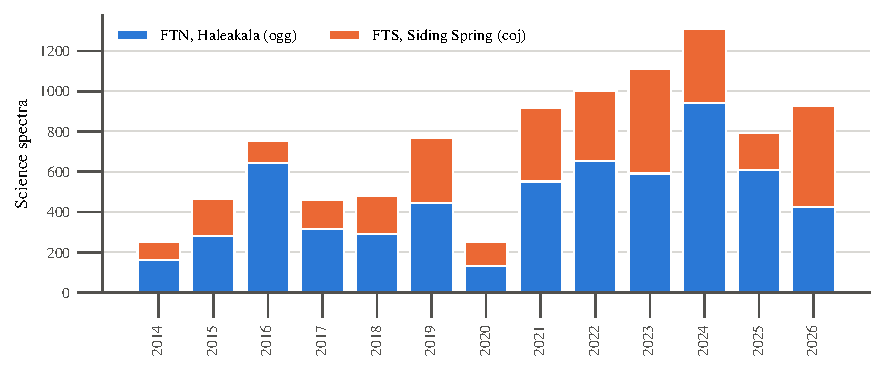
\includegraphics[width=\textwidth]{figures/fig_spectra_year.pdf}
\caption{FLOYDS science spectra per year and telescope.}\label{fig:spectra}
\end{figure}

\section{Arcs and lamp flats}
Each raw spectrum (science and standards) is linked to the arcs and lamp flats on the same spectrograph within
seven days, ranked by: same observing block, then same slit width, then time; the best three of each type are
kept (\texttt{calib\_match}). The best arc comes from the same block for \fracArcBlock\,\% of the spectra and the
best lamp flat for \fracFlatBlock\,\%; \nNoArc{} spectra have no arc within seven days.

\section{Flux standards}\label{sec:standards}
The key projects took few standards of their own. The standards were therefore collected by name from any
proposal: observatory calibration programmes (\texttt{COJ\_calib}, \texttt{OGG\_calib}, \texttt{FLOYDS standards},
engineering) and other key projects, \nStdFrames{} spectra of \nStdTargets{} stars from \nStdProposals{}
proposals (Table~\ref{tab:standards}). For each science spectrum the five nearest standards of each slit width
on the same spectrograph are kept, with a standard in the same block ranked first (\texttt{std\_match}). The
nearest standard is a median of \medStdDt~h away (Fig.~\ref{fig:stddt}); a standard with the same slit width
exists for \fracSameSlit\,\% of the spectra, a median of \medStdDtSame~d away. Most observatory standards are
taken with the 2-arcsec slit while the science uses 6 arcsec, which is the main limitation for the flux calibration.

The standard used for each science spectrum (view \texttt{spectrum\_standards}) is chosen in this order: the
nearest standard taken with the same slit width; failing that, the nearest standard taken with the 2-arcsec slit;
failing that, the nearest standard with any slit (a standard in the same block always wins over time). The three
cases apply to \nPickSame, \nPickTwo{} and \nPickAny{} science spectra, and \nPickNone{} have no standard on the same
spectrograph within 30~d. Spectra whose headers are not yet in the database have no known slit width and fall in
the second or third case.

\begin{figure}[h]
\centering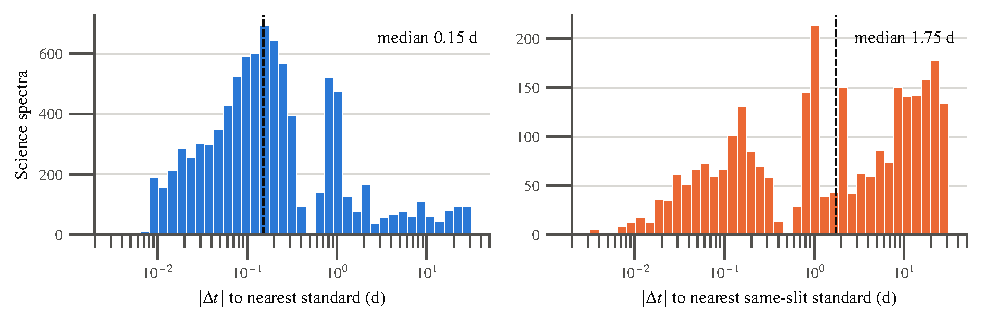
\includegraphics[width=\textwidth]{figures/fig_std_dt.pdf}
\caption{Time to the nearest standard (left) and to the nearest standard with the same slit width (right).}\label{fig:stddt}
\end{figure}

\begin{small}
\begin{longtable}{lrlrrp{5.2cm}}
\caption{Flux standards in the spectra database: number of spectra, date range, slit widths, number of science
spectra for which it is the selected standard, and the proposals they come from.}\label{tab:standards}\\
\toprule
Star & N & Dates & Slits & Best for & Proposals \\
\midrule\endfirsthead
\toprule
Star & N & Dates & Slits & Best for & Proposals \\
\midrule\endhead
\inputtable{tables/tab_standards.tex}
\bottomrule
\end{longtable}
\end{small}
